%!TEX options=--shell-escape
\documentclass[tikz]{standalone}
\usepackage[T1]{fontenc}
\usepackage[utf8]{inputenc}
\usepackage{xcolor}
\usepackage{amsmath}
\usepackage{amssymb}
\usepackage{hyperref}
\usepackage{accsupp}    
\usepackage{graphicx}
\usepackage{mathtools}
\usepackage{pagecolor}
\usepackage{amsmath} % for \dfrac
\usepackage{tikz}
\tikzset{>=latex} % for LaTeX arrow head
\usepackage{braket}
\usepackage{pgfplots} 
\usepackage[edges]{forest}
\usetikzlibrary{patterns, backgrounds, arrows.meta}
\setlength{\parindent}{0cm}
\setlength{\parskip}{1em}

\usetikzlibrary{patterns}
\def\rescale{0.142857}
\def\offset{0.035}

\begin{document}
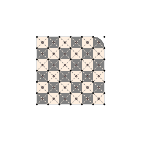
\begin{tikzpicture}[scale=\rescale]

   \foreach \y in {0,2,...,4}{
    \foreach \x in {0,2,...,3}{
        \fill[gray] (\x,\y) rectangle (1+\x,1+\y);
        \fill[gray] (\x + 1,\y + 1) rectangle (2+\x,2+\y);

        \fill[yellow!40!red!10] (\x+1,\y) rectangle (\x+2,\y+1);
        \fill[yellow!40!red!10] (\x,\y+1) rectangle (\x+1,\y+2);
    }}

   \foreach \y in {0,2,...,4}{
    \foreach \x in {4}{
        \fill[gray] (\x,\y) rectangle (1+\x,1+\y);
        \fill[yellow!40!red!10] (\x,\y+1) rectangle (\x+1,\y+2);
    }}

   \foreach \y in {0,2,...,3}{
    \foreach \x in {5}{
        \fill[gray] (\x,\y+1) rectangle (1+\x,2+\y);
        \fill[yellow!40!red!10] (\x,\y) rectangle (\x+1,\y+1);
    }}
    \fill[yellow!40!red!10] (5,4) rectangle (6,5);
    \fill[gray] (5,5) -- (5,6) to [bend left=45](6, 5) -- cycle;

    \foreach \x in {0, 1, ...,5}{
        \foreach \y in {0, 1, ...,5}{
            \filldraw[line width = \rescale, draw=black, fill=pink!60] (\x + 0.5, \y + 0.5) circle[radius=2pt] node[font=\tiny] {};
        }
    }


    % X Lattice
    \foreach \x in {0, 2, ..., 5}{
            \draw[line width = \rescale, dash pattern={on 0.5pt off 0.5pt on 0.5pt off 0.5pt}, gray] (\x, 0) -- (0, \x);
            \draw[line width = \rescale, dash pattern={on 0.5pt off 0.5pt on 0.5pt off 0.5pt}, gray] (\x, 6) -- (6, \x);
            \draw[line width = \rescale, dash pattern={on 0.5pt off 0.5pt on 0.5pt off 0.5pt}, gray] (\x + 1, 6) -- (0, 5 - \x);
            \draw[line width = \rescale, dash pattern={on 0.5pt off 0.5pt on 0.5pt off 0.5pt}, gray] (\x + 1, 0) -- (6, 5 - \x);
%            \draw[line width = 0.25*\rescale, dash pattern={on 0.5pt off 0.5pt on 0.5pt off 0.5pt}, gray] (0, \x + 0.5) -- (0, \x);
%            \draw[line width = 0.25*\rescale, dash pattern={on 0.5pt off 0.5pt on 0.5pt off 0.5pt}, gray] (6, \x + 1) -- (6, \x + 2);
    }

    % Z Lattice
    \foreach \x in {1, 3, ..., 4}{
            \draw[line width = \rescale, dash pattern={on 0.5pt off 0.5pt on 0.5pt off 0.5pt}, yellow!40!red!10] (0, \x) -- (\x,0);
            \draw[line width = \rescale, dash pattern={on 0.5pt off 0.5pt on 0.5pt off 0.5pt}, yellow!40!red!10] (\x, 6) -- (6, \x);
            \draw[line width = \rescale, dash pattern={on 0.5pt off 0.5pt on 0.5pt off 0.5pt}, yellow!40!red!10] (\x + 1, 6) -- (0, 5 - \x);
            \draw[line width = \rescale, dash pattern={on 0.5pt off 0.5pt on 0.5pt off 0.5pt}, yellow!40!red!10] (\x + 1, 0) -- (6, 5 - \x);
%            \draw[line width = 0.25*\rescale, dash pattern={on 0.5pt off 0.5pt on 0.5pt off 0.5pt}, yellow!40!red!10] (\x, 0) -- (\x + 1, 0);
%            \draw[line width = 0.25*\rescale, dash pattern={on 0.5pt off 0.5pt on 0.5pt off 0.5pt}, yellow!40!red!10] (\x, 6) -- (\x - 1 , 6);
    }
    \draw[line width = \rescale, dash pattern={on 0.5pt off 0.5pt on 0.5pt off 0.5pt}, yellow!40!red!10] (0, 0) -- (5.5,5.5);
    \draw[line width = \rescale, dash pattern={on 0.5pt off 0.5pt on 0.5pt off 0.5pt}, yellow!40!red!10] (0, 5) -- (5,0);

    % Corner tiles
    \draw[line width = \rescale, dash pattern={on 0.5pt off 0.5pt on 0.5pt off 0.5pt}, yellow!40!red!10] (5, 6) to (5.5,5.5);
    \draw[line width = \rescale, dash pattern={on 0.5pt off 0.5pt on 0.5pt off 0.5pt}, yellow!40!red!10] (6, 5) to (5.5,5.5);


    \foreach \x in {0, 1, ...,5}{
        \foreach \y in {0, 1, ...,5}{
            \filldraw[line width=0.25*\rescale, draw=black, fill=pink!60] (\x + 0.5, \y + 0.5) circle[radius=2pt] node[font=\tiny] {};
        }
    }



    \foreach \x in {0, 1, ...,6}{
        \foreach \y in {0, 1, ...,6}{
            \filldraw[line width=0.25*\rescale, draw=black] (\x, \y) circle[radius=2pt] node[font=\tiny] {};
        }
    }
    \draw[line width=0.25*\rescale] (0, 0) -- (6, 0) -- (6, 5) to [bend right=45] (5, 6) -- (0, 6) -- (0, 0);

\end{tikzpicture} 
\end{document}

